\subsection{Ground Sample Distance - GSD}
In order to associate image properties with real life properties, one can use what is known as Ground Sample Distance. This is a way to express and measure what one pixel in the image represents in the real world. The result will be a scaling factor given in $[m/pixel]$, where we can use this factor to scale pixel values to meter values.\\

Ground Sample Distance can be viewed as a measure of resolution limitations of an image sensor due to sampling\cite{s}. Assuming the sensor is pointed normal to the ground, it is in effect a measure of the real-world distance between two pixel centers on the ground. The angular distance between sensor samples is given by pixel pitch $p$ divided by focal length of the sensor $f$. Assuming this angular distance is projected on the ground, it defines GSD:
\begin{figure}
  \centering
  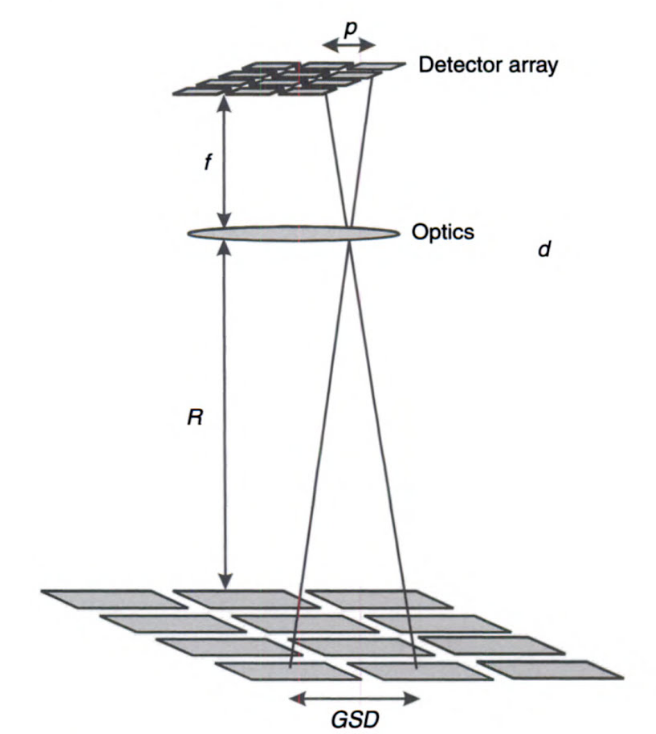
\includegraphics[width=0.7\textwidth]{fig/GSDimage}
  \caption{Ground Sample Distance. From \cite{s}}
  \label{fig:gsd}
\end{figure}
\begin{align}
    GSD = \frac{p}{fW}R \quad\quad\textrm{[meters/pixel]}
    \label{gsd1}
\end{align}
Where $R$ is the distance from the optics to the ground and $W$ is the width of the image in pixels. GSD is illustrated in Figure \ref{fig:gsd}. Equation \ref{gsd1} assumes that the sensor is directed normal to the ground surface. If this is not the case, the GSD must be corrected for the look angle between the ground and the sensor $\theta$:
\begin{align}
    GSD = \frac{pR}{fW\cos{\theta}}\quad\quad\textrm{[meters/pixel]}
    \label{gsd2}
\end{align}
Where $\theta$ is the angle the sensor is facing normal to the ground. It is important to note that there are two different GSD's, one in the horizontal and one in the vertical direction. By taking the geometric mean of the horizontal and vertical ground sample distances you get a two-dimensional system GSD\cite{s}.